\documentclass[tikz, landscape]{standalone}
\usepackage[charter]{mathdesign}
\usetikzlibrary{arrows, arrows.meta, automata, positioning}
\tikzset{larrow/.style = {-{Latex[length=.5em]}}}

\begin{document}
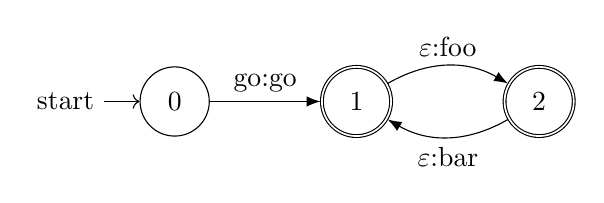
\begin{tikzpicture}
    \node[state,initial] (0) at (0,0) {0};
    \node[state,accepting] (1) [right=4em of 0] {1};
    \node[state,accepting] (2) [right=4em of 1] {2};

    \draw[larrow] (0) to node [above] {go:go} (1);
    \draw[larrow,bend left] (1) to node [above] {$\varepsilon$:foo} (2);
    \draw[larrow,bend left] (2) to node [below] {$\varepsilon$:bar} (1);
\end{tikzpicture}
\end{document}
